\section{Isolated Benzene}
    In order to verify if our new implementations work as intended, we compare the spectral functions we obtain for the isolated benzene ring with the one obtained by F. Hörbinger via exact diagonalisation of the PPP model \cite{hoerbinger}. We find that our results shown in Fig. \ref{fig:isolated_benzene} match those from \cite{hoerbinger} up to three significant figures, after conversion into the appropriate units. Thus we can be fairly confident that our implementation works, at least for the isolated Benzene system.

\medskip
\begin{figure}[!hbt]
    \centering
    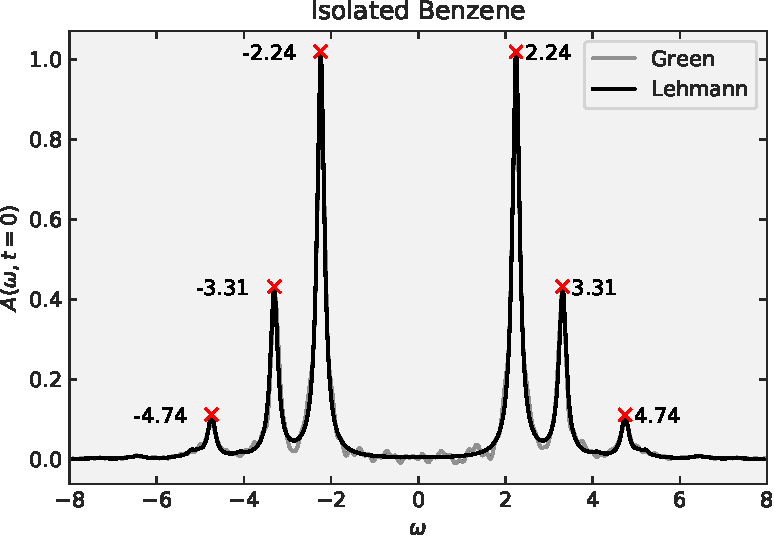
\includegraphics[width=0.7\textwidth]{graph/isolated_benzene.pdf}
    \caption{Spectral function of isolated benzene with peak energies in agreement with results from \cite{hoerbinger}\newline
    Parameters: $U = 3.96$, $a = 0.3$, $t_0 = 0$, broadening-factor $\epsilon = 0.1 $
    }\label{fig:isolated_benzene}
\end{figure}

Additionally we can also see from Fig. \ref{fig:isolated_benzene} that both the Lehmann spectrum and the spectral function obtained via the Fourier transformation of the Green's function produce comparable results, the only differences being the ``noise" that is introduced in the Greens function spectrum due to the Fourier transform. This could be suppressed further by tweaking the broadening factor and the zero-padding of the domain, as briefly described in \ref{sec:spectral_functions}.